\documentclass{article}

% if you need to pass options to natbib, use, e.g.:
%     \PassOptionsToPackage{numbers, compress}{natbib}
% before loading neurips_2019

% ready for submission
% \usepackage{neurips_2019}

% to compile a preprint version, e.g., for submission to arXiv, add add the
% [preprint] option:
%     \usepackage[preprint]{neurips_2019}

% to compile a camera-ready version, add the [final] option, e.g.:
     \usepackage[final]{neurips_2019}

% to avoid loading the natbib package, add option nonatbib:
%     \usepackage[nonatbib]{neurips_2019}

\usepackage[utf8]{inputenc} % allow utf-8 input
\usepackage[T1]{fontenc}    % use 8-bit T1 fonts
\usepackage{hyperref}       % hyperlinks
\usepackage{url}            % simple URL typesetting
\usepackage{booktabs}       % professional-quality tables
\usepackage{amsfonts}       % blackboard math symbols
\usepackage{nicefrac}       % compact symbols for 1/2, etc.
\usepackage{microtype}      % microtypography
\usepackage{graphicx}

\title{Formatting Instructions For NeurIPS 2019}

% The \author macro works with any number of authors. There are two commands
% used to separate the names and addresses of multiple authors: \And and \AND.
%
% Using \And between authors leaves it to LaTeX to determine where to break the
% lines. Using \AND forces a line break at that point. So, if LaTeX puts 3 of 4
% authors names on the first line, and the last on the second line, try using
% \AND instead of \And before the third author name.

\author{%
  Luke Oakden-Rayner\\
  %\thanks{Use footnote for providing further information
    %about author (webpage, alternative address)---\emph{not} for acknowledging
    %funding agencies.} \\
  School of Public Health\\
  University of Adelaide\\
  Adelaide, SA 5000 \\
  \texttt{luke.oakden-rayner@adelaide.edu.au} \\
  \And
%\author{%
    Jared Dunnmon\\
  %\thanks{Use footnote for providing further information
    %about author (webpage, alternative address)---\emph{not} for acknowledging
    %funding agencies.} \\
  Department of Computer Science\\
  Stanford University\\
  Stanford, CA 94305 \\
  \texttt{jdunnmon@stanford.edu} \\
  \And
  Christopher R\'{e}\\
  %\thanks{Use footnote for providing further information
    %about author (webpage, alternative address)---\emph{not} for acknowledging
    %funding agencies.} \\
  Department of Computer Science\\
  Stanford University\\
  Stanford, CA 94305 \\
  \texttt{chrismre@stanford.edu } \\
  \And
    Lyle Palmer\\
  %\thanks{Use footnote for providing further information
    %about author (webpage, alternative address)---\emph{not} for acknowledging
    %funding agencies.} \\
  School of Public Health\\
  University of Adelaide\\
  Adelaide, SA 5000 \\
  \texttt{lyle.palmer@adelaide.edu.au} } 
  % examples of more authors
  % \And
  % Coauthor \\
  % Affiliation \\
  % Address \\
  % \texttt{email} \\
  % \AND
  % Coauthor \\
  % Affiliation \\
  % Address \\
  % \texttt{email} \\
  % \And
  % Coauthor \\
  % Affiliation \\
  % Address \\
  % \texttt{email} \\
  % \And
  % Coauthor \\
  % Affiliation \\
  % Address \\
  % \texttt{email} \\
%}

\begin{document}

\maketitle

\begin{abstract}
Machine learning models for medical image analysis often suffer from poor performance on important subsets of a population that are not identified at train time.  
We refer to this problem as \textit{hidden stratification}, and observe that it results from incomplete schema that do not describe the full space of meaningful variation in a dataset.  
While hidden stratification can substantially affect the clinical utility of machine learning models, its effects remain difficult to measure because comprehensive schema are difficult to prescribe.
In this work, we assess the utility of two existing techniques for measuring hidden stratification effects -- schema completion and error auditing -- on multiple medical imaging datasets, and observe that hidden stratification results in performance differences of up to 20\% on clinically important subsets.
We further propose a simple unsupervised algorithm for measuring hidden stratification, and present evidence that such algorithmic measurement approaches could help to detect hidden stratification in practice.
Finally, we explore the clinical implications of our findings, and discuss processes by which hidden stratification could be accounted for in both model development and deployment for medical imaging applications. 
\end{abstract}

\section{Introduction}

Deep learning systems have shown remarkable promise in medical image analysis, often performing at a similar level to human experts in various tasks. 
 However, performance results reported in the literature may overstate the clinical utility and safety of these models.  
 Specifically, it is well known that machine learning models often make mistakes that humans never would, despite having aggregate error rates comparable to or better than those of human experts. 
 This property of machine learning models is often of little significance in non-medical tasks where safety is not critical and all errors are roughly equivalent in cost, but in medical practice the specific errors made can have serious clinical impacts. 
 
Of particular concern is the fact that most medical machine learning models are built and tested using incomplete label schema, where the training labels only coarsely describe the meaningful variation within the population. 
Medical images contain dense visual information, and imaging diagnoses are usually identified by recognising the combination of several different visual features or patterns. 
This means that any given pathology or variant is actually comprised of several visually and clinically distinct subgroups; a ``lung cancer'' label, for example, would contain both solid and subsolid tumours, as well as central and peripheral neoplasms. 
We call this phenomenon \textit{hidden stratification}, meaning that the data contains unrecognised subsets of cases which may affect model training, model performance, and most importantly the clinical outcomes related to the use of a medical image analysis system.  

Worryingly, when these subsets are not labelled, test performance may be falsely reassuring. 
This is because the test performance (an aggregate measure such as sensitivity or ROC AUC) can be dominated by larger subsets, obscuring the fact that there is an unidentified subset of cases within which performance is poor. 
Given the rough medical truism that serious diseases are less common than mild diseases, it is even likely that underperformance in minority subsets could lead to disproportionate harm to patients.

While the effects of hidden stratification have been known in the machine learning community for some time, they remain difficult to measure. 
 Even if it is not yet apparent how to solve hidden stratification problems in practice, we argue that measurement of these effects should be a critical component of machine learning deployments in medicine.  
 One methodologically straightforward approach is what we call \textit{schema completion}.  
 Schema completion entails prospective delineation of a label schema that reflects the full range of meaningful variations in a population.  
 In practice, schema completion is difficult in medical imaging not only because it requires a great deal of both annotation effort and clinical insight, but also because artifacts routinely appear in clinical practice that can invalidate existing schemas (e.g. chest tubes, hardware artifacts, visual effects of new treatments, new pathology subclasses, etc.).  
 Another potential approach is retrospective \textit{error auditing}, where the results of machine learning models are consistently evaluated by domain experts to identify meaningful hidden stratification effects in deployed models.  
 While error auditing is useful, the expertise and attentiveness of the auditor is crucial to audit efficacy.  
 A third potential approach involves unsupervised measurement techniques, where algorithmic interrogation of the model can indicate the presence of hidden stratification effects.  Unfortunately, this class of techniques remains relatively underdeveloped.

In this article, we demonstrate that hidden stratification is a fundamental technical problem that should be considered when applying machine learning algorithms to medical imaging analysis.  
We illustrate that hidden stratification is present both in standard computer vision models trained on the CIFAR-100 benchmark dataset and in three different machine learning applications in projection radiography.  
We initially demonstrate the utility of two different techniques for measuring hidden stratification effects -- schema completion and error auditing -- and observe that  hidden stratification results in performance differences of up to 20\% on clinically important subsets.  
We further propose an unsupervised clustering approach that can assist practitioners in identifying when hidden stratification may substantially impact model performance, and assess its performance on these datasets.
We examine the clinical implications of these findings in detail, and discuss mechanisms by which hidden stratification could be effectively measured within clinical workflows.

\section{Related Work}

The difficulty of this hidden stratification problem is fundamentally related to the challenge of obtaining labelled training data.  
Were fine-grained labels available for every clinical variant of importance, it would be feasible to train and evaluate models using this information.  
Typical approaches to observed stratification and dataset imbalance in medical machine learning often center on gathering much data as possible on underperforming subsets, either via additional labelling, selective data augmentation, or oversampling (Mazurowski et al. 2008).  
However, the cost of manual labelling is often prohibitive, appropriate augmentation transforms can be difficult to define, and oversampling an underperforming subset can cause degradation on others (Fries et al. 2019; Ratner et al. 2017; Agniel, Kohane, and Weber 2018; Buda, Maki, and Mazurowski 2018; Zech et al. 2018).  
As a result, rather than exhaustively labelling all possible findings and variations in medical images, teams have begun to perform either semi-automated labelling (X. Wang et al. 2017; Irvin et al. 2019; Chilamkurthy et al. 2018; J. Dunnmon et al. 2019; Fries et al. 2019) or have applied human expertise to produce a narrow or incomplete set of visual labels, which often exhibit reduced accuracy (Oakden-Rayner 2019).  
While such approaches have shown promise, techniques that reliably increase performance on critical subsets without degrading performance on others have yet to be demonstrated.
 
Methods that directly address hidden stratification, where the subclasses are obscure, have not been widely explored in medical imaging analysis.  However, it is clear from the recent literature that this issue has been widely (but not universally) recognised.  
(Gulshan et al. 2016), for instance, present variations in retinopathy detection performance on subsets with images obtained in different locations, subsets with differing levels of disease severity, and subsets of images with different degrees of pupil dilation.  
In several cases, their models perform differently on these subsets in a manner that would be clinically impactful.  (Chilamkurthy et al. 2018)  present a subset analysis for different diagnostic categories of intracranial haemorrhage (e.g. subdural vs subarachnoid) when designing a deep learning model for abnormality detection on head CT, but do not analyze differences in  performance related to bleed size, location, or the appearance of the bleed (ie acute vs subacute). 
 These workers, do, however, evaluate the performance of models on cases with multiple findings, and observe substantial variation in model performance within different strata; for instance, subarachnoid bleed detection performance appears to degrade substantially in the presence of an epidural hemorrhage.  
 (P. Wang et al. 2019) perform an excellent subset analysis of a colonscopy polyp detector, with comparative performance analysis presented by polyp size, location, shape, and underlying pathology (e.g. adenoma versus hyperplastic).  
 Similarly, (J. A. Dunnmon et al. 2019) report the performance of their chest radiograph triage system by pathology subtype, finding that models trained on binary triage labels achieved substantially lower performance on fracture than on other diseases.   
 Multiple workers also find that non-causal confounding variables such as hospital process quantities contribute substantially to high model performance on data subsets heavily associated with these confounding variables  (Winkler et al. 2019; Badgeley et al. 2019; Agniel et al. 2018; Zech et al. 2018).  
 Other studies perform error audits, where specific failure modes such as small volume cancers, disease mimics, and chest hardware are observed (Taylor, Mielke, and Mongan 2018; Campanella et al. 2019); such analyses may be helpful in identifying obvious error modes via human review, but do not characterize the full space of subset performance (Selbst 2017).  
 Of course, there also exist multiple studies that do not directly address the effects of hidden stratification (Haenssle et al. 2018; Bien et al. 2018). 
 (Esteva et al. 2017) is particularly notable, as this study does present findings for carcinoma and melanoma subclasses, and dermatoscopic images vs photographs, but does not report performance for any of the more than 2,000 diagnostic subclasses they define in their label schema -- analysis of these effects would improve the community?s ability to assess the real-world clinical utility of these models. 
 
Perhaps the most well-developed literature describing methods that address problems similar to hidden stratification is that describing fairness and bias in machine learning systems. 
 Technically, this subfield is concerned with ensuring that machine learning systems perform in ways that align with social goals such as avoiding discrimination based on sensitive features or providing equal opportunity to all users of a system (Barocas, Hardt, and Narayanan 2017).  
 The work of (Selbst 2017) is of particular relevance to hidden stratification in medical imaging, as they identify several different mechanisms by which machine learning algorithms can end up performing differently for different subsets of the population. 
  The first of these is that of skewed examples.  
  In this situation, for example, a training dataset initially contains far more positives from one subset than another.  
  When the resulting model is deployed, it leads to additional observations that that reinforce performance on the original high-performing subset at the expense of performance on other subsets. 
  Tainted examples, on the other hand, refer to the situation when the quantity used as the ground truth (e.g. past hiring decisions) does not directly measure the quantity of interest (e.g. future performance of a job applicant).  
  (Selbst 2017) also propose that both sample size disparity between subsets and limited discriminative features between subsets can result in reduced performance. 
   Finally, the idea of proxies -- features that are correlated with the outcome of interest, but not causal -- is identified as a determining factor in differential subset performance. 
    Each of these situations can occur in the context of medical imaging systems, and methods developed by such workers as  (Hardt et al. 2016; Zafar et al. 2017) for addressing the results of these fundamental issues of bias and fairness should be explored further in medical imaging.  

\section{Measuring Hidden Stratification}

We propose that there exist three broad approaches to mitigate the clinical risk of hidden stratification: 1) exhaustive human labeling of the data, called schema completion, 2) human analysis of model predictions, called subset analysis or audit, and 3) algorithmic methods to detect hidden strata. These methods are applied to the test dataset, allowing for the reporting of model performance in previously hidden strata.  We describe each of these approaches in detail below.  

\subsection{Schema Completion}
The schema author (usually the developer) prospectively decides what subclasses need to be labeled, and performs this task on test data. Any report of model performance (ie for regulatory approval) would include both superclass and subclass performance results. 
This is dependent on domain knowledge, to pre-emptively identify all subclasses deemed to be important. 

Strengths: prospective, can develop consensus on ?important? subclasses for a given task (e.g. a professional body could produce standards describing reporting expectations). Can guide model development (with knowledge of difficult cases).

Weaknesses: limited by subclass ?expectations?, so if there are important subclasses that are not included in the schema, then schema completion does not protect against clinical failure. Time consuming to exhaustively label subclasses (diagnostic, demographic, clinical, descriptive, etc).

Example: The MURA experiments in this study were relabeled with a consensus schema produced by a team of radiologists (unpublished). This schema focused on diagnostic (ie fracture, arthritis) and hospital process (ie metalwork) categories, and did not cover descriptive or location based categories (ie displaced fracture, radiocarpal arthritis).
The hip fracture experiments were relabeled with a schema developed by LOR, including both location (subcapital, cervical etc) and descriptive (mildly displaced, comminuted etc) categories.

\subsection{Error Auditing}
The auditor (may be developers or external testing agents) examine the model outputs for unexpected regularities, for example a difference in the distribution of a recognisable subclass in the correct and incorrect model predictions groups. 
This process is dependent on both domain knowledge and image interpretation. 

Strengths: not limited by expectations, the subclasses identified are directly related to model function. 

Weaknesses: depends on being able to visually recognise differences in the distribution of model outputs (ie correct and incorrect superclass predictions). In particular almost impossible to identify low prevalence high discordance subsets (since they rarely occur, so noting presence/absence in visually assessed cases is challenging). The non-exhaustive nature of audit may limit certainty that all hidden strata were analysed, for example in the setting of regulatory approval.

Example: The CXR14 experiments were performed by analysing the model predictions, where it was discovered that the false negative pneumothorax cases were far less likely to contain chest drains than the

\subsection{Algorithmic Approaches}
The algorithm developer designs a method to look for subclasses automatically. 
This will usually be an unsupervised method such as clustering. If any identified group (ie a cluster) underperforms compared to the superclass, then this may indicate the presence of a clinically relevant subclass, which will then require human review to characterise (similar to audit, but targeted by the algorithm). 

Strengths: automated, reduces burden on human labelers. Data-driven.

Weaknesses: limited by separability of data, it is likely that many subclasses will not separate after clustering, resulting in incomplete reporting of hidden strata.

Example: We include results of simple k-means clustering below.

\section{Experiments}

In our experiments, we empirically measure the effect of hidden stratification on a benchmark computer vision dataset as well as onthree different medical imaging datasets from projection radiography.  We leverage schema completion or error auditing to measure these effects in each case and further investigate an unsupervised clustering-based method to assist in identifying the presence of poorly-performing subsets.  In the following Discussion section, we analyze the clinical implications of these results and evaluate approaches by which hidden stratification might be measured or addressed within medical imaging workflows.

\subsection{Datasets}

\subsection{Schema Completion}

We first demonstrate the utility of schema completion by measuring the effects of hidden stratification on CIFAR-100, MURA, and Hip Fracture Datasets.

\subsubsection{CIFAR-100}

The benchmark CIFAR-100 dataset from computer vision represents an excellent testbed on which to demonstrate the effect of hidden stratification in a well-characterized environment (Krizhevsky, Nair, and Hinton 2009).  
The CIFAR-100 dataset consists of 60,000 images binned into 20 ?superclasses,? which each contain five distinct ?subclasses.? 
 Each subclass is represented in the dataset with equal frequency.  
 We hypothesize that by training models only on superclass labels, and assessing superclass performance within each subclass, we will commonly observe subclasses on which performance is substantially inferior to that of the overall superclass.  
 We further expect that subclass performance will degrade if a given subclass is subsampled or if noise is added to superclass labels for a given subclass.  
 While we do not explicitly evaluate the effect of visually similar subclasses or spurious correlates on CIFAR-100, we expect that similar effects would be observed.  
 Because we assume that the CIFAR-100 subclasses represent a comprehensive schema, we implement schema completion by measuring superclass accuracy within each subclass.
 
 Table \ref{tab:cifar1} below shows the results on specific subclasses and superclasses when 75\% of the examples in a specific subclass are dropped from the training set.  While the overall marine mammals superclass performance drops by only 4 accuracy points when the dolphin subclass is subsampled in this way, performance on the dolphin subclass (with respect to the superclass label) drops by 14 points from 0.78 (9 points above overall superclass performance) to 0.64 (1 point below overall superclass performance).  Similar trends are observed for the mountain subclass.  Clearly, unmeasured subclass underrepresentation can lead to substantially worse performance on that subclass, even when superclass performance is only modestly affected.
 
Table \ref{tab:cifar2} shows a similar trend when noise is added to a given subclass, which simulates lower label quality on that subclass.  We observe that performance on both dolphin and mountain subclasses drop substantially when label accuracy decreases.  Such stratification of label quality by pathology is highly likely to occur in medical datasets, where certain pathologies are easier to identify than others.

 \begin{figure}[htb!]
 \centering
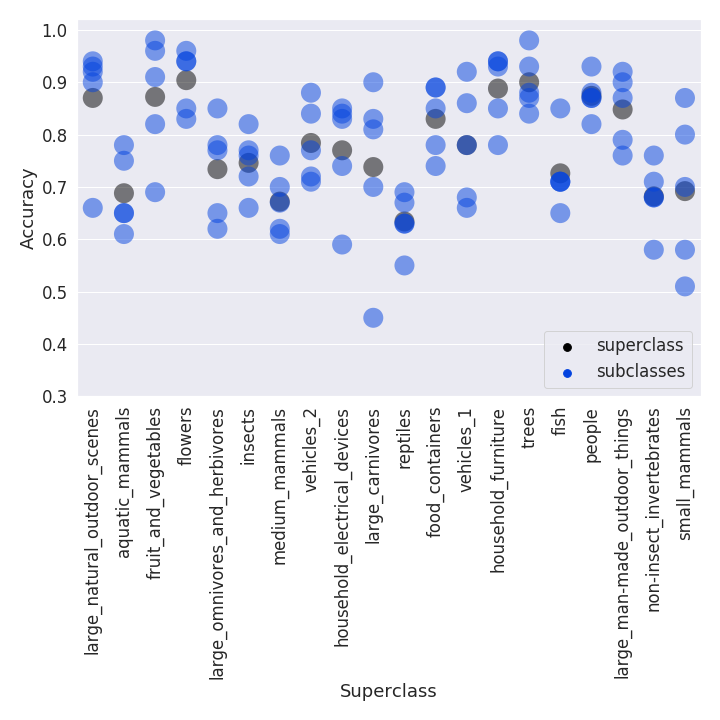
\includegraphics[width=5in]{Superclass-Subclass-CIFAR-100-Correct-Val-v2.png}
\label{fig:cifar}
\caption{Performance of ResNeXt-29, 8x64d on CIFAR-100 superclasses by subclass.  Note that most superclasses contain subclasses where performance is far lower than that on the aggregate superclass.  This same phenomenon occurs in medical imaging datasets, and can have substantial effects on how these models would be deployed in practice.}
\end{figure}

\begin{table}[]
\begin{tabular}{ccccc}
 Subclass & Baseline Superclass  & Baseline Subclass  & 25\% Subsample Superclass  & 25\% Subsample Subclass \\
 Dolphin & 0.69 & 0.78  & 0.65  & 0.64  \\
 Mountain & 0.87 & 0.90  & 0.82 & 0.71  \\
\end{tabular}
\label{tab:cifar1}
\caption{Accuracy of ResNeXt-29, 8x64d trained using the full CIFAR-100 dataset (``Baseline'') and a modified dataset (``Subsample'') where 75\% of the Dolphin and Mountain subclasses were dropped from the training dataset.  All results reported are with respect to the superclass label.}
\end{table}

\begin{table}[]
\begin{tabular}{ccccc}
 Subclass & Baseline Superclass  & Baseline Subclass  & 25\% Whiten Superclass  & 25\% Whiten Subclass \\
 Dolphin & 0.69 & 0.78  & 0.65  & 0.64  \\
 Mountain & 0.87 & 0.90  & 0.82 & 0.71  \\
\end{tabular}
\label{tab:cifar2}
\caption{Accuracy of ResNeXt-29, 8x64d trained using the full CIFAR-100 dataset (``Baseline'') and a modified dataset (``Whiten'') where 25\% of the examples in the Dolphin and Mountain subclasses were assigned a random superclass label.  All results reported are with respect to the superclass label.
}
\end{table}

Figure \ref{fig:cifar} presents the performance of a ResNeXt-29, 8x64d CNN trained on the 20 CIFAR-100 superclasses using the training schedule reported in (Xie et al. 2016) and the implementation provided by (Yang n.d.).  
In each superclass, the five constituent subclasses exhibit substantial performance variation, and in some cases the worst-performing subclass underperforms the aggregate superclass by over 30 accuracy points.  
This same phenomenon in medical imaging would lead to massively different outcomes for different subsets of the population, be these demographically or pathologically determined.  

\subsubsection{MURA}

MURA is a musculoskeletal x-ray dataset developed by (Rajpurkar et al. 2017), which provides labels for a single class, identifying cases that are ?normal? and ?abnormal?. 
These labels were produced by radiologists in the course of their normal work, and include various visually distinct abnormalities including fractures, implanted metal, bone tumours, and degenerative joint disease. 
These labels have been previously investigated and relabelled by a board certified radiologist (Oakden-Rayner 2019), showing significant differences in both the prevalence and accuracy of the labels within several of these subclasses. 
The distribution of these subclasses is shown in Table \ref{tab:mura1}.


\begin{table}[]
\begin{tabular}{ccc}
 Subclass & Subclass Prevalence & Sensitivity \\
 Fracture & 0.30 & 0.92   \\
 Metalwork & 0.11 & 0.85    \\
 Degenerative Change & 0.43 & 0.60 
\end{tabular}
\label{tab:mura1}
\caption{MURA ?abnormal? label prevalence and sensitivity for the subclasses of ?fracture?, ?metalwork?, and ?degenerative joint disease.? The degenerative disease subclass labels have the highest prevalence but the lowest accuracy.}
\end{table}

For MURA, we hypothesize that the label quality for the degenerative disease subclass will result in reduced performance on that subclass, and that the visually obvious metalwork subclass will have high performance (despite low prevalence).
 We train a DenseNet-169 was trained on the normal/abnormal labels, with XX cases used for training and YY cases held-out for testing.  
 We test the model on aggregate labels, as well as by subclass.  
 We assess ROC-AUC values for the model on each subclass and in aggregate as a proxy for model performance; results are presented below in Figure \ref{fig:mura}.  
 We find that overall AUC for the easy-to-detect hardware subclass (0.96) is higher than aggregate AUC (0.88), while performance on clinically important fracture and degenerative  disease subsets are substantially lower.  
 In this case, we measure hidden stratification using schema completion, as radiologists have a good understanding of what important subsets may exist in extremity radiographs.

 \begin{figure}[htb!]
 \centering
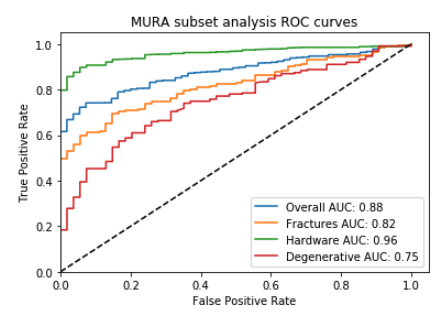
\includegraphics[width=3in]{MURA-ROC-temp.png}
\label{fig:mura}
\caption{ROC curves for model performance different subclasses of the abnormal superclass.}
\end{figure}

\subsubsection{Hip Fracture}

As a third clinical task, we analyze a large, high quality pelvic x-ray dataset produced at the Royal Adelaide Hospital.
 A Densenet model trained on this dataset to identify hip fractures achieved extremely high performance (AUC = 0.994). 
 This previously trained binary hip fracture detection model predicted the presence or absence of a fracture on the validation and test sets, using the threshold defined in (Gale et al. 2017).  
 The distribution of the location and description subclasses is shown in Table 6, with subclass labels produced by a board-certified radiologist.  
 We hypothesize that reduced subclass performance will occur even in models with very high overall superclass performance, particularly in subclasses characterised by ?subtle? visual features.  
 Again, because this particular diagnostic is clinically well-characterized, we use schema completion to measure the effects of hidden stratification.  
 We assess sensitivity values for the model on each subclass and in aggregate as a proxy for model performance at detecting fractures.  
 We find that sensitivity on subclasses such as cervical, subtrochanteric, and subtle fractures are significantly lower than that on both other subsets and the overall superclass.  
 
\begin{table}[]
\centering
\begin{tabular}{ccc}
 Subclass & Subclass Prevalence & Sensitivity \\
 Overall & - & 0.981  \\
 Subcapital & 156 & 0.987   \\
 Cervical & 79 & \textbf{0.911}\\
 Pertrochanteric & 315  & 0.997\\
 Subtrochanteric & 23 & \textbf{0.957} \\
 Subtle & 20 & \textbf{0.900}\\
 Mildly Displaced & 172 & 0.983\\
 Moderately Displaced & 192 & 1.000\\
 Severely Displaced & 228 & 0.996\\
 Commuted & 169 & 1.000 \\ 
\end{tabular}
\label{tab:hip1}
\caption{Superclass and subclass performance for hip fracture detection from frontal pelvic x-rays. Bolded subclasses demonstrate significantly worse performance than the closest/most similar class(es).}
\end{table}

\subsection{Error Audit}

\subsubsection{CXR-14}

We next use the CXR-14 dataset as an example of how error auditing can be used to detect the effects of hidden stratification in a real clinical application

The CXR-14 dataset is a large-scale dataset for pathology detection in chest radiographs (Wang et al. 2017). 
This dataset was released in 2017 and updated later the same year, containing 112,120 frontal chest films from 30,805 unique patients. 
The dataset is drawn from a single tertiary medical centre (the NIH Clinical Center) and appears to include films from multiple clinical settings, including intensive care unit (ICU) and non-ICU patients.  
Each image was labeled for one of 14 different thoracic pathologies.  
In our analysis, we leverage a pretrained Densenet-121 model provided by (Zech) which reproduces the procedure and results of (Rajpurkar et al. 2018) on this dataset.  

During error auditing of pretrained model results, it was observed that the model was performing particularly well on examples within the pneumothorax class that contained chest drains. 
 As a result, pneumothorax subclass labels for ?chest drain? and ?no chest drain? were provided by a board-certified radiologist (LOR) for each element of the test set.  
 Due to higher prevalence of scans with chest drains in the dataset, clear discriminative features of a chest drain, and high label quality for the scans with chest drains, we hypothesize that a model trained on the CXR-14 dataset will attain higher performance on the pneumothorax subclass with chest drains than that without chest drains.  
 
 \begin{table}[]
 \centering
\begin{tabular}{ccc}
 Subclass & Subclass Prevalence & Sensitivity \\
 Chest Drain & 0.80 & 0.90   \\
 No Chest Drain & 0.20 & 0.60    
\end{tabular}
\label{tab:mura1}
\caption{ CXR14 ``pneumothorax'' label prevalence and positive predictive value for the subclasses ``with chest drain'' and ``without chest drain''. Cases without chest drains are both the minority, as well as labelled with reduced accuracy (determined by visual inspection).}
\end{table}

 We present the prevalence of each subclass and positive predictive values of the pretrained model on those subsets in Table \ref{tab:cxr14-1} and ROC curves for each subclass in Figure \ref{fig:cxr14}.  
 We find that 80\% of the pneumothorax examples in the test set contained a test drain, and that positive predictive value on this subset was 30\% higher than on those without a chest drain.  
 Further, we find that while the ROC-AUC of the pretrained model closely matched that reported in the literature at 0.87, the model achieved an ROC-AUC value of 0.94 on the subclass with chest drains, but only 0.77 on the subclass without chest drains.  
 These results demonstrate that hospital process variables can create subclasses with obvious features that form a majority of the pneumothorax superclass, substantially lowering performance on identifying the clinically important subclass of pneumothoraces without chest drains.  
 Note that while we present results obtained from a pretrained model, analysis using a model trained from scratch yielded equivalent results. 

 \begin{figure}[htb!]
 \centering
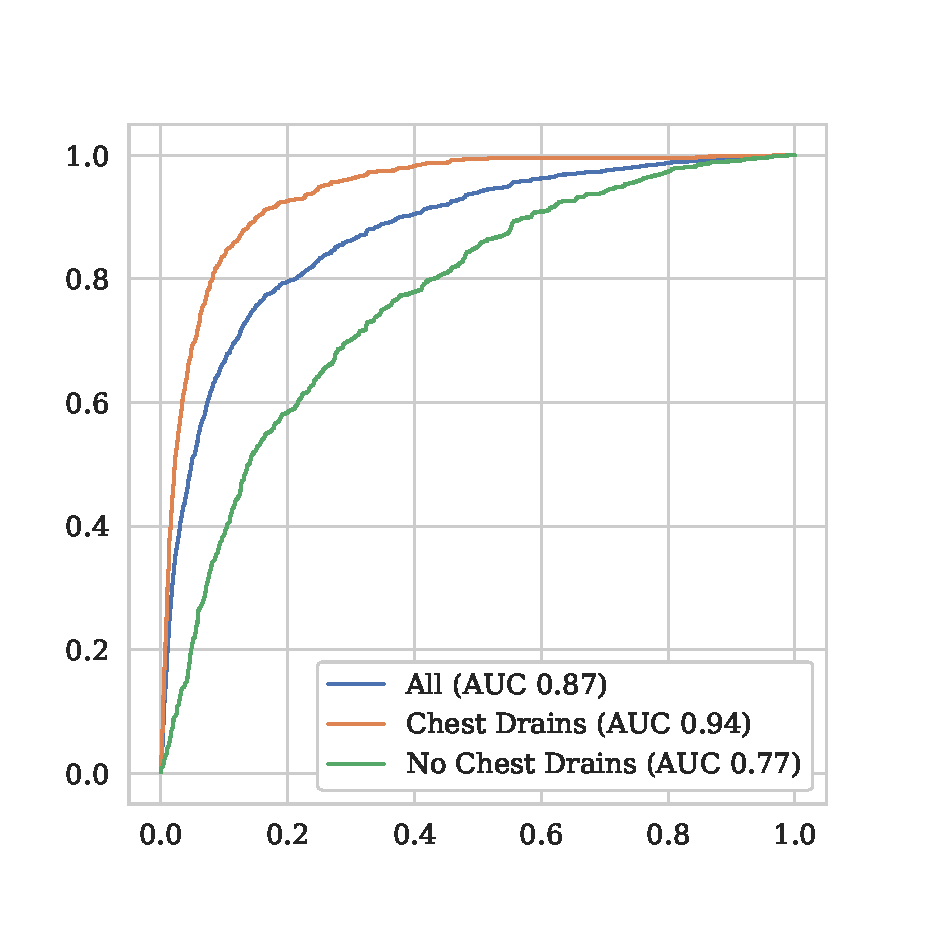
\includegraphics[width=3in]{Pneumo-ROC.eps}
\label{fig:cxr14}
\caption{ROC curves for model performance on different subclasses of the pneumothorax superclass.}
\end{figure}

\subsection{Algorithmic Approaches: Unsupervised Clustering}

We also perform an unsupervised clustering procedure to identify the presence of hidden stratification. *ARE THESE NORMALIZED BY SIZE?*


 \begin{table}[]
 \centering
\begin{tabular}{cccc}
 Clustering Method & Difference in Error (High Error, Low Error) & Difference in Prevalence (High Error, Low Error) & Inter-cluster Distance \\
 Hidden State Only & 0.57 (0.59, 0.02) & 0.30 (0.36, 0.06) & 4.0 \\
 Error Only & 0.89 (0.91, 0.02) & 0.33 (0.40, 0.07) & 0.9 \\
 Error-weighted Hidden State & 0.70 (0.78, 0.08) & 0.26 (0.38, 0.12) & 3.7
\end{tabular}
\label{tab:clustercifar-1}
\caption{ CIFAR-100.}
\end{table}

 \begin{table}[]
 \centering
\begin{tabular}{cccc}
 Clustering Method & Difference in Error (High Error, Low Error) & Difference in Prevalence (High Error, Low Error) & Inter-cluster Distance \\
 Hidden State Only & 0.43 (0.96, 0.53) & 0.68 (0.17, 0.84) & 12.1 \\
 Error Only & 0.68 (0.96, 0.27) & 0.58 (0.34, 0.92) & 0.7 \\
 Error-weighted Hidden State & 0.51 (0.97, 0.46) & 0.77 (0.13, 0.90) & 13.9
\end{tabular}
\label{tab:clustercxr14-1}
\caption{ CXR-14.}
\end{table}

 \begin{table}[]
 \centering
\begin{tabular}{cccc}
 Clustering Method & Difference in Error (High Error, Low Error) & Difference in Prevalence (High Error, Low Error) & Inter-cluster Distance \\
 Hidden State Only & 0.05 (0.49, 0.54) & 0.03 (0.26, 0.29) & 16.2 \\
 Error Only & 0.84 (0.05, 0.89) & 0.34 (0.13, 0.47) & 0.8 \\
 Error-weighted Hidden State & 0.58 (0.23, 0.81) & 0.27 (0.15, 0.42) & 7.22
\end{tabular}
\label{tab:clustermura-1}
\caption{ MURA.}
\end{table}

% \begin{table}[]
% \centering
%\begin{tabular}{cccc}
% Clustering Method & Difference in Error (High Error, Low Error) & Difference in Prevalence (High Error, Low Error) & Inter-cluster Distance \\
% Hidden State Only & 0.43 (0.96, 0.53) & 0.68 (0.17, 0.84) & 12.1 \\
% Error Only & 0.68 (0.96, 0.27) & 0.58 (0.34, 0.92) & 0.7 \\
% Error-weighted Hidden State & 0.51 (0.97, 0.46) & 0.77 (0.13, 0.90) & 13.9
%\end{tabular}
%\label{tab:clustercxr14-1}
%\caption{ TBD.}
%\end{table}
%
% \begin{table}[]
% \centering
%\begin{tabular}{cccc}
% Clustering Method & Difference in Error (High Error, Low Error) & Difference in Prevalence (High Error, Low Error) & Inter-cluster Distance \\
% Hidden State Only & 0.43 (0.96, 0.53) & 0.68 (0.17, 0.84) & 12.1 \\
% Error Only & 0.68 (0.96, 0.27) & 0.58 (0.34, 0.92) & 0.7 \\
% Error-weighted Hidden State & 0.51 (0.97, 0.46) & 0.77 (0.13, 0.90) & 13.9
%\end{tabular}
%\label{tab:clustercxr14-1}
%\caption{ TBD.}
%\end{table}
%
% \begin{table}[]
% \centering
%\begin{tabular}{cccc}
% Clustering Method & Difference in Error (High Error, Low Error) & Difference in Prevalence (High Error, Low Error) & Inter-cluster Distance \\
% Hidden State Only & 0.43 (0.96, 0.53) & 0.68 (0.17, 0.84) & 12.1 \\
% Error Only & 0.68 (0.96, 0.27) & 0.58 (0.34, 0.92) & 0.7 \\
% Error-weighted Hidden State & 0.51 (0.97, 0.46) & 0.77 (0.13, 0.90) & 13.9
%\end{tabular}
%\label{tab:clustercxr14-1}
%\caption{ TBD.}
%\end{table}
%
% \begin{table}[]
% \centering
%\begin{tabular}{cccc}
% Clustering Method & Difference in Error (High Error, Low Error) & Difference in Prevalence (High Error, Low Error) & Inter-cluster Distance \\
% Hidden State Only & 0.43 (0.96, 0.53) & 0.68 (0.17, 0.84) & 12.1 \\
% Error Only & 0.68 (0.96, 0.27) & 0.58 (0.34, 0.92) & 0.7 \\
% Error-weighted Hidden State & 0.51 (0.97, 0.46) & 0.77 (0.13, 0.90) & 13.9
%\end{tabular}
%\label{tab:clustercxr14-1}
%\caption{ TBD.}
%\end{table}

\section{Discussion}

Our results show that hidden stratification can lead to markedly different primary task and subclass performance, both when the labels for the subclasses have different levels of accuracy and when the subclasses are imbalanced.  
We observe this to be the case in both a controlled CIFAR-100 environment and on multiple clinical datasets.

The clinical implications of this phenomenon will vary by clinical task. In our experiments, the MURA results are unlikely to be clinically relevant, because degenerative disease is rarely a significant or unexpected finding, nor are rapid complications likely. 
We can hypothesise that labels derived from clinical practice are likely to demonstrate this phenomenon; that irrelevant or unimportant findings are often elided by radiologists because they are unimportant, leading to reduced label quality for the less significant findings.

The findings in the CXR14 task are far more concerning. 
The majority of x-rays in the dataset contain chest drains, which is in effect a hospital process variable that is not causally linked to pneumothorax diagnosis.
 Importantly, the presence of a chest drain means these pneumothorax cases are already treated and are therefore at almost no risk of pneumothorax-related harm. 
 In this experiment, we see that the performance in the clinically important subclass of cases without chest drains is far worse than the primary task results would suggest. 
 We could easily imagine a situation where a model is justified for clinical use or regulatory approval with the results from the primary task alone, as the images used for testing simply reflect the clinical set of patients with pneumothoraces.
 
While this example is quite extreme, this does correspond with the medical truism that serious disease is typically less common than non-serious disease. 
This may suggest that in many medical scenarios, image analysis systems that appear to perform well in a given task may fail to identify the most clinically important cases. 
This is particularly concerning when comparing these systems to human experts, who tend to focus a lot of effort on specifically learning to identify rare, dangerous, and subtle disease variants.

The performance of medical image analysis systems is unlikely to be fully explained by the prevalence and accuracy of the labels, or even the dataset size. 
In the MURA experiment, the detection of metalwork is vastly more accurate than the detection of fractures or degenerative change, despite this subclass being both smaller and less accurately labelled than fractures. 
We hypothesise that the nature of the visual features is important as well; metalwork is highly visible and discrete, as metal is significantly more dense (with higher pixel values) than any other material on x-ray. 
While our understanding of what types of visual features are more learnable than others is limited, it is not unreasonable to assume that detecting metal in an xray is far easier for a deep learning model than identifying a subtle fracture (and particularly on downsampled images).

Similarly, chest drains are highly recognisable in pneumothorax imaging, and small untreated pneumothoraces are subtle enough to be commonly missed by radiologists. 
It is possible that this effect exaggerates the discrepancy in performance on the pneumothorax detection task, beyond the effect of subclass imbalance alone.

Our simple approach to identify unrecognised subgroups in our training and test appears to work well across a variety of tasks, and produces XXX . 
This technique could be considered a first attempt at easing the burden of human visual review needed to assess clinical image analysis systems. 
Interestingly the naive approach that clusters cases using the hidden state only performs nearly as well as the error-weighted clustering, suggesting again that deep learning models do learn semantically meaningful differences between subclasses, even if performance is not equal across these. 
This supports other findings that demonstrate the utility of hidden-state clustering in deep learning model development (Liu et al. 2019).

It remains to be seen if these automatically produced clusters can be useful in practice, either for finding clinical important subclasses or for use in retraining image analysis models for improved subclass performance. 
More advanced methods may be required to tackle this problem, or it may be the case that unsupervised or semi-supervised approaches are unable to contribute substantially, leaving us reliant on time-consuming methodical human review.
These experiments do not explore the full range of medical image analysis tasks, and as such the results will have variable applicability to any given scenario.
 These findings are intended to highlight this largely unrecognised problem, suggesting that awareness of hidden stratification is important and should be considered (even if to be dismissed) when planning, building, and regulating clinical image analysis systems.
 
 **SUGGEST METHODS FOR INTEGRATION INTO ACTUAL WORKFLOWS**


\section{Conclusion}

Hidden stratification in medical image datasets appears to be a significant and under-appreciated problem. Not only can the unrecognised presence of visual subclasses lead to impaired subclass performance, but this may even result in unexpected negative clinical outcomes in situations where image analysis models silently fail to learn serious but rare, noisy, or subtle visual subclasses.
Acknowledging the presence of visual variation within class labels is likely to be important when building and evaluating medical image analysis systems.
**DISPARATE IMPACT VS. DISPARATE TREATMENT** -- mention fairness/bias stuff here, ditto with slicing


\section*{Acknowledgments}

\section*{References}


\end{document}
